\documentclass[12pt,a4paper]{article}
% Fix for fancyhdr headheight error
\setlength{\headheight}{14.5pt}
% --- PACKAGES ---
% --- ENCODING & FONTS ---
\usepackage[utf8]{inputenc}
\usepackage[T1]{fontenc}
\usepackage{lmodern}          % Modern font (alternative to Times)
% \usepackage{times}          % OPTIONAL: Classic serif font (comment if using lmodern)

\usepackage{pgf-pie}
\usepackage{pgfplots}
\usepackage{subcaption}
\usepackage{xcolor}
\usepackage{colortbl}
\usepackage{multirow}
\usepackage{booktabs}
\usepackage{siunitx}
\usepackage{float}

% --- PAGE LAYOUT ---
\usepackage[a4paper, left=0.75in, right=0.75in, top=1in, bottom=1in]{geometry}
\usepackage{parskip}          % Paragraphs with spacing instead of indentation
\usepackage{setspace}         % For line spacing

% --- MATHEMATICS ---
\usepackage{amsmath, amsfonts, amssymb}

% --- GRAPHICS & FIGURES ---
\usepackage{graphicx}
\usepackage{caption}
\usepackage{float}
\usepackage{array, longtable, colortbl}
\usepackage{tabularx}

% --- COLORS ---
\usepackage[table]{xcolor}
\usepackage{xcolor}           % General color usage

% --- TIKZ & DIAGRAMS ---
\usepackage{tikz}
\usetikzlibrary{
  shapes.geometric,
  arrows.meta,
  positioning,
  fit,
  backgrounds,
  shapes.multipart
}

% --- PLOTS & CHARTS ---
\usepackage{pgf-pie}          % Pie charts
\usepackage{pgfplots}         % Graphs and plots
% Set pgfplots compatibility for modern features
\pgfplotsset{compat=1.18}

% --- DOCUMENT STRUCTURE ---
\usepackage{titlesec}         % Custom section titles
\usepackage{tocloft}          % Table of contents formatting
\usepackage{enumitem}         % Better lists

% --- HEADER, FOOTER & LINKS ---
\usepackage{fancyhdr}         % Custom headers/footers

% --- BIBLIOGRAPHY ---
\usepackage[numbers,sort&compress]{natbib}  % For references with numerical citations
\bibliographystyle{plainnat}  % Compatible style with natbib
\usepackage[many]{tcolorbox}
\tcbuselibrary{skins,breakable}

% --- Code listings for source code in Appendix ---
\usepackage{listings}
\lstset{
    language=Python,
    basicstyle=\ttfamily\small,
    breaklines=true,
    showstringspaces=false,
    numbers=left,
    numberstyle=\tiny\color{gray},
    frame=single,
    captionpos=b,
    keywordstyle=\color{blue},
    commentstyle=\color{green!60!black},
    stringstyle=\color{purple},
    rulecolor=\color{black!20},
    backgroundcolor=\color{black!5}
}

% --- Load hyperref last ---
\usepackage{hyperref}         % Clickable links


% --- COLORS ---
\definecolor{RoyalBlue}{RGB}{0, 70, 140}
\definecolor{RUETRed}{RGB}{179, 0, 0}
\definecolor{LightGray}{RGB}{248, 249, 250}
\definecolor{DarkGray}{RGB}{52, 58, 64}
\definecolor{AccentBlue}{RGB}{13, 110, 253}
\definecolor{ModernGray}{RGB}{108, 117, 125}
\definecolor{lightgreen}{RGB}{200, 255, 200}
\definecolor{lightred}{RGB}{255, 200, 200}

% Define modern color palette
\definecolor{primary}{RGB}{41, 128, 185}
\definecolor{secondary}{RGB}{52, 152, 219}
\definecolor{accent}{RGB}{231, 76, 60}
\definecolor{success}{RGB}{46, 204, 113}
\definecolor{warning}{RGB}{241, 196, 15}
\definecolor{darkgray}{RGB}{52, 73, 94}
\definecolor{lightgray}{RGB}{236, 240, 241}
\definecolor{purple}{RGB}{155, 89, 182}
\definecolor{orange}{RGB}{230, 126, 34}
\definecolor{teal}{RGB}{26, 188, 156}
\definecolor{OliveGreen}{RGB}{85, 107, 47}

\definecolor{outputbg}{RGB}{45, 45, 45} % Dark background for output

% --> ADDED for the blue info box
% --> Define colors for code boxes and result boxes
\definecolor{reportgreen}{RGB}{230, 245, 230}
\definecolor{reportdarkgreen}{RGB}{50, 120, 50}
\definecolor{outputbg}{RGB}{45, 45, 45} % Dark background for output
\definecolor{infoboxbg}{RGB}{235, 245, 255}
\definecolor{infoboxborder}{RGB}{70, 130, 180}
% --> ADDED: Define the blue info box style
\newtcolorbox{infobox}{
  colback=infoboxbg,
  colframe=infoboxborder,
  boxrule=0.5pt, % thin border for sides/bottom
  borderline north={1.5pt}{0pt}{infoboxborder}, % thicker top border
  arc=0mm,       % sharp corners
  left=5mm, % Add some padding
  top=3mm,
  bottom=3mm
}

% --> Define style for code listings (like Listing 2, 3 in friend's report)
\lstdefinestyle{code}{
    basicstyle=\ttfamily\small,
    numbers=left,
    numberstyle=\tiny\color{gray},
    numbersep=5pt,
    frame=none,
    breaklines=true,
    keywordstyle=\color{blue},
    commentstyle=\color{OliveGreen},
    stringstyle=\color{purple},
    showstringspaces=false
}
\lstset{style=code} % Set default listing style

% --> Define the green result box
\newtcolorbox{resultbox}[2][]{
    enhanced,
    attach boxed title to top center={yshift=-2mm},
    colback=reportgreen,
    colframe=reportdarkgreen,
    colbacktitle=reportgreen,
    coltitle=black,
    boxed title style={size=small,colframe=reportdarkgreen},
    title={#2},
    fonttitle=\bfseries
}

% --- FONT & STYLING ---
\renewcommand{\familydefault}{\sfdefault}  % Use sans-serif font
\titleformat{\section}{\fontsize{20}{24}\selectfont\bfseries\color{RoyalBlue}}{\thesection}{1em}{}
\titleformat{\subsection}{\fontsize{16}{20}\selectfont\bfseries\color{RoyalBlue}}{\thesubsection}{1em}{}
\titleformat{\subsubsection}{\fontsize{13}{16}\selectfont\bfseries\color{RoyalBlue}}{\thesubsubsection}{1em}{}

% TOC Styling
\renewcommand{\cfttoctitlefont}{\color{black}\Huge\bfseries}
\renewcommand{\cftsecfont}{\color{RoyalBlue}}
\renewcommand{\cftsecpagefont}{\color{RoyalBlue}}
\renewcommand{\cftsubsecfont}{\color{RoyalBlue}}
\renewcommand{\cftsubsecpagefont}{\color{RoyalBlue}}

% Header and Footer
\pagestyle{fancy}
\fancyhf{}
\fancyhead[C]{\textit{Compiler Design Sessional}}
\fancyfoot[C]{\thepage}
\renewcommand{\headrulewidth}{0.4pt}
\renewcommand{\footrulewidth}{0pt}

% Hyperlink Styling
\hypersetup{
    colorlinks=true,
    linkcolor=RoyalBlue,
    filecolor=magenta,
    urlcolor=cyan,
    pdftitle={Data Mining Report},
    pdfpagemode=FullScreen,
    pdfborder={0 0 0},
}

% --- Define a global style for all plots for consistency ---
\pgfplotsset{
    every axis/.append style={
        axis x line=bottom,
        axis y line=left,
        label style={font=\bfseries},
        title style={font=\large\bfseries, yshift=1em},
        tick label style={font=\small},
        legend style={font=\small, at={(0.5,-0.2)}, anchor=north, legend columns=-1},
    }
}

% Modern title page with geometric design
\newcommand{\maketitlepage}{
    \begin{titlepage}
        \begin{tikzpicture}[remember picture,overlay]
            \fill[RoyalBlue!10] (current page.north west) rectangle ([yshift=-2.2cm]current page.north east);
            \fill[AccentBlue!5] ([yshift=-14cm]current page.north west) rectangle ([yshift=-16.2cm]current page.north east);
            \fill[RoyalBlue!15] ([xshift=2cm,yshift=-2cm]current page.north west) circle (1.2cm);
            \fill[AccentBlue!15] ([xshift=-2cm,yshift=-15.2cm]current page.north east) circle (0.9cm);
        \end{tikzpicture}

        \centering
        \vspace*{0.6cm}

        % Logo (only include if file exists)
        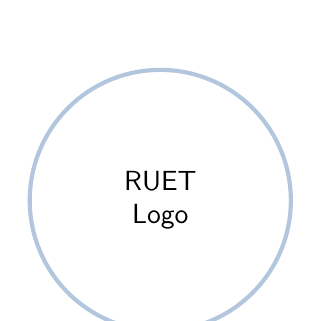
\begin{tikzpicture}
            \node[circle, draw=RoyalBlue!30, line width=1.5pt, inner sep=6pt] at (0,0) {
                 \IfFileExists{RUET_logo.png}{\includegraphics[width=2.7cm]{RUET_logo.png}}{\begin{minipage}{2.7cm}\centering RUET \\ Logo \end{minipage}}
            };
        \end{tikzpicture}

        \vspace{0.6cm}
        {\fontsize{15.5}{17}\selectfont\bfseries\textcolor{RUETRed}{RAJSHAHI UNIVERSITY OF ENGINEERING \& TECHNOLOGY}\par}
        \vspace{0.2cm}
        {\fontsize{13.5}{16}\selectfont\textcolor{DarkGray}{Department of Computer Science and Engineering}\par}

        \vspace{1.5cm}
        % Title Block
        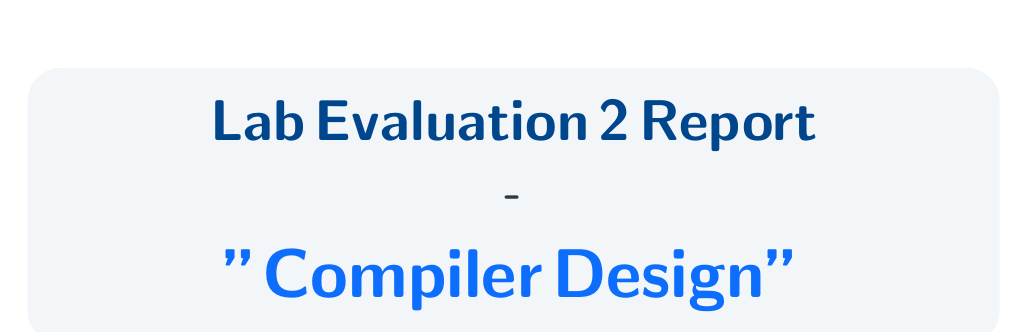
\begin{tikzpicture}
            \node[rectangle, fill=RoyalBlue!5, rounded corners=12pt, inner sep=12pt, text width=11.5cm, align=center] at (0,0) {
                {\fontsize{21}{24}\selectfont\bfseries\textcolor{RoyalBlue}{Lab Evaluation 2 Report}\par}
                \vspace{0.15cm}
                {\fontsize{16}{20}\selectfont\bfseries\textcolor{DarkGray}{-}\par}
                \vspace{0.15cm}
                {\fontsize{24}{28}\selectfont\bfseries\textcolor{AccentBlue}{"Compiler Design"}\par}
            };
        \end{tikzpicture}

        \vspace{1.8cm}
        % Submission info
        \begin{minipage}[t]{0.45\textwidth}
            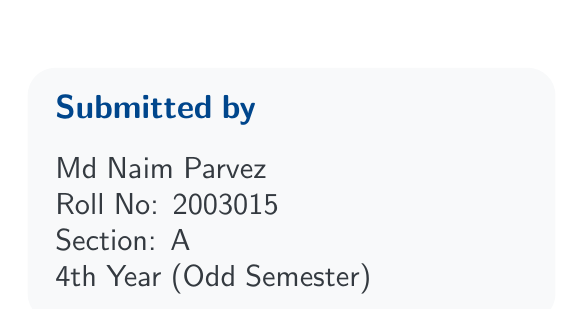
\begin{tikzpicture}
                \node[rectangle, fill=LightGray, rounded corners=10pt, inner sep=10pt, text width=6cm] at (0,0) {
                    {\fontsize{13}{15}\selectfont\bfseries\textcolor{RoyalBlue}{Submitted by}\par}
                    \vspace{0.3cm}
                    {\fontsize{11}{13}\selectfont\textcolor{DarkGray}{
                        Md Naim Parvez\\
                        Roll No: 2003015\\
                        Section: A\\
                        4th Year (Odd Semester)
                    }\par}
                };
            \end{tikzpicture}
        \end{minipage}
        \hfill
        \begin{minipage}[t]{0.50\textwidth}
            
\begin{tikzpicture}
                \node[rectangle, fill=AccentBlue!5, rounded corners=10pt, inner sep=10pt, text width=6cm] at (0,0) {
                    {\fontsize{13}{15}\selectfont\bfseries\textcolor{RoyalBlue}{Submitted to}\par}
                    \vspace{0.3cm}
                    {\fontsize{11}{13}\selectfont\textcolor{DarkGray}{
                        Farjana Parvin\\
                        Assistant Professor\\
                        Department of CSE\\
                        Rajshahi University of Engineering \& Technology\\
                        \vspace{0.3cm}
                    }\par}
                };
            \end{tikzpicture}
        \end{minipage}

        \vspace{1.2cm}
        % Course Info
        
\begin{tikzpicture}
            \node[rectangle, fill=RoyalBlue!10, rounded corners=10pt, inner sep=12pt, align=center, text width=13cm] at (0,0) {
                {\fontsize{13}{16}\selectfont\bfseries\textcolor{RoyalBlue}{Course Code: } \textcolor{DarkGray}{4102}}\\[0.2cm]
                {\fontsize{13}{16}\selectfont\bfseries\textcolor{RoyalBlue}{Course Title: } \textcolor{DarkGray}{Compiler Design Sessional}}
            };
        \end{tikzpicture}

        \vspace{0.8cm}
    \end{titlepage}
}


\begin{document}

% --- TITLE PAGE ---
\maketitlepage
\thispagestyle{empty} % No header/footer on the title page

\newpage
% --- TABLE OF CONTENTS ---
\pagenumbering{roman} % Roman numerals for ToC, Abstract etc.
\phantomsection % Helps hyperref create proper links
\tableofcontents

% --- LIST OF FIGURES ---
\newpage
\phantomsection % Helps hyperref create proper links
\pagenumbering{arabic} % Arabic numerals for main content
\setcounter{page}{1} % Start main content page numbering from 1

\section{Introduction}

Compiler design is a fundamental area of computer science that bridges the gap between high-level programming languages and machine-executable code. At the heart of any compiler lies two critical phases: lexical analysis and syntax analysis. These phases transform raw source code into a structured representation that can be further processed for semantic analysis, optimization, and code generation.

\subsection{Background}
Lexical analysis, also known as scanning or tokenization, is the first phase of compilation. It reads the source code as a stream of characters and groups them into meaningful sequences called tokens. Each token represents a basic syntactic unit such as keywords, identifiers, operators, or literals. This process simplifies the subsequent parsing phase by reducing the complexity of character-level processing.

Syntax analysis, or parsing, follows lexical analysis and verifies that the sequence of tokens conforms to the grammatical rules of the programming language. It constructs a parse tree or abstract syntax tree (AST) that represents the hierarchical structure of the source code. This tree serves as the foundation for semantic analysis and code generation phases.


\section{Objective}
The objective of this laboratory exercise is to:
\begin{enumerate}
    \item Understand lexical analysis using Flex (Fast Lexical Analyzer)
    \item Implement syntax analysis using Bison (Parser Generator)
    \item Tokenize and parse structured statements containing year and degree information
    \item Demonstrate the integration of lexer and parser for language processing
\end{enumerate}

\section{Theory}

\subsection{Lexical Analysis (Flex)}
Lexical analysis is the first phase of compilation where the source code is converted into a sequence of tokens. Flex is a tool for generating scanners (lexical analyzers) that recognize lexical patterns in text.

\textbf{Key Components:}
\begin{itemize}
    \item \textbf{Tokens:} Basic building blocks (keywords, identifiers, numbers, operators)
    \item \textbf{Patterns:} Regular expressions that define token recognition rules
    \item \textbf{Actions:} C code executed when a pattern is matched
\end{itemize}

\subsection{Syntax Analysis (Bison)}
Syntax analysis (parsing) is the second phase of compilation where tokens are organized into a parse tree according to grammar rules. Bison is a parser generator that produces LALR(1) parsers from context-free grammar specifications.

\textbf{Key Components:}
\begin{itemize}
    \item \textbf{Grammar Rules:} Define the structure of valid statements
    \item \textbf{Terminal Symbols:} Tokens from the lexer
    \item \textbf{Non-terminal Symbols:} Abstract syntactic constructs
    \item \textbf{Semantic Actions:} Code executed when rules are reduced
\end{itemize}

\subsection{Flex-Bison Integration}
Flex and Bison work together in the compilation pipeline:
\begin{enumerate}
    \item Flex generates \texttt{lex.yy.c} (lexical analyzer)
    \item Bison generates \texttt{code1.tab.c} and \texttt{code1.tab.h} (parser and token definitions)
    \item Both are compiled together to create the final parser
    \item The parser reads input, tokenizes it via Flex, and validates structure via Bison
\end{enumerate}

\section{Problem Statement}
Given statements in the format:
\begin{verbatim}
Year (2020) MBA-3
Year (2019) MSc-2
Year (2022) BBA-1
\end{verbatim}

\textbf{Tasks:}
\begin{enumerate}
    \item Create a Flex file (\texttt{code1.l}) to tokenize these statements
    \item Create a Bison file (\texttt{code1.y}) to parse the tokenized input
    \item Demonstrate successful parsing with detailed output
\end{enumerate}

\section{Input Data}

\subsection{Input File (input.txt)}
\begin{lstlisting}[caption={Input statements for parsing}]
Year (2020) MBA-3  
Year (2019) MSc-2  
Year (2022) BBA-1
\end{lstlisting}

\section{Implementation}

\subsection{Flex File (code1.l)}
The lexical analyzer defines patterns for recognizing tokens:

\begin{lstlisting}[language=C, caption={code1.l - Flex Lexical Analyzer}]
%{
#include <stdio.h>
#include <stdlib.h>
#include <string.h>
#include "code1.tab.h"
%}
%%
"Year"                  { 
    printf("%s -> KEYWORD\n", yytext);
    yylval.str = strdup(yytext); 
    return KEYWORD; 
}
"MBA"|"MSc"|"BBA"|"BSc"|"PhD"|"MA"|"BA"   { 
    printf("%s -> DEGREE_NAME\n", yytext);
    yylval.str = strdup(yytext); 
    return DEGREE; 
}
[0-9]+                  { 
    printf("%s -> NUMBER\n", yytext);
    yylval.num = atoi(yytext); 
    return NUMBER; 
}
"("                     { 
    printf("( -> LPAREN\n");
    return LPAREN; 
}
")"                     { 
    printf(") -> RPAREN\n");
    return RPAREN; 
}
"-"                     { 
    printf("- -> DASH\n");
    return DASH; 
}
[ \t]+                  { /* ignore whitespace */ }
\n                      { 
    printf("\\n -> NEWLINE\n");
    return NEWLINE; 
}
.                       { 
    printf("%c -> UNKNOWN\n", yytext[0]);
    return yytext[0]; 
}
%%
int yywrap() {
    return 1;
}
\end{lstlisting}

\subsection{Token Definitions}
\begin{table}[h]
\centering
\begin{tabular}{|l|l|l|}
\hline
\textbf{Pattern} & \textbf{Token} & \textbf{Description} \\
\hline
"Year" & KEYWORD & Reserved keyword \\
"MBA"|"MSc"|"BBA" & DEGREE & Degree program names \\
{[}0-9{]}+ & NUMBER & Numeric values \\
"(" & LPAREN & Left parenthesis \\
")" & RPAREN & Right parenthesis \\
"-" & DASH & Hyphen/dash character \\
\textbackslash n & NEWLINE & Line terminator \\
{[ }\textbackslash t{]}+ & - & Whitespace (ignored) \\
\hline
\end{tabular}
\caption{Token patterns and their recognition rules}
\end{table}

\subsection{Bison File (code1.y)}
The parser defines grammar rules for statement validation:

\begin{lstlisting}[language=C, caption={code1.y - Bison Parser Specification}]
%{
#include <stdio.h>
#include <stdlib.h>
#include <string.h>
int yylex();
void yyerror(const char *s);
%}
%union {
    char *str;
    int num;
}
%token <str> KEYWORD DEGREE
%token <num> NUMBER
%token LPAREN RPAREN DASH NEWLINE
%%
program:
    line_list
    ;
line_list:
    line
    | line_list line
    ;
line:
    year_statement NEWLINE
    | NEWLINE
    ;
year_statement:
    KEYWORD LPAREN NUMBER RPAREN DEGREE DASH NUMBER
    {
        printf("Parsed: Year (%d) %s-%d\n", $3, $5, $7);
    }
    ;
%%
int main(){
    printf("Starting parser for year and degree information...\n");
    
    yyparse();
    printf("Parsing Finished\n");
    return 0;
}
void yyerror(const char *s){
    printf("Timestamp: %s %s\n error: %s\n", __DATE__, __TIME__, s);
}
\end{lstlisting}

\subsection{Grammar Rules Explanation}

\textbf{Production Rules:}
\begin{verbatim}
program → line_list
line_list → line | line_list line
line → year_statement NEWLINE | NEWLINE
year_statement → KEYWORD LPAREN NUMBER RPAREN DEGREE DASH NUMBER
\end{verbatim}

\textbf{Rule Descriptions:}
\begin{itemize}
    \item \textbf{program:} Starting symbol, consists of one or more lines
    \item \textbf{line\_list:} Handles multiple lines recursively
    \item \textbf{line:} Each line is either a year statement or empty
    \item \textbf{year\_statement:} Matches the pattern "Year (YYYY) DEGREE-N"
\end{itemize}

\subsection{Makefile}
\begin{lstlisting}[language=make, caption={Makefile for Building Parser}]
main: code1.l code1.y
	bison -d code1.y
	flex code1.l
	gcc code1.tab.c lex.yy.c
	./a.out <input.txt> output.txt
\end{lstlisting}

\textbf{Build Process:}
\begin{enumerate}
    \item \texttt{bison -d code1.y} - Generates parser (\texttt{code1.tab.c}) and header (\texttt{code1.tab.h})
    \item \texttt{flex code1.l} - Generates lexer (\texttt{lex.yy.c})
    \item \texttt{gcc code1.tab.c lex.yy.c} - Compiles and links both components
    \item \texttt{./a.out <input.txt> output.txt} - Runs parser with input redirection
\end{enumerate}

\section{Execution and Results}

\subsection{Compilation Steps}
\begin{verbatim}
$ make
bison -d code1.y
flex code1.l
gcc code1.tab.c lex.yy.c
./a.out <input.txt> output.txt
\end{verbatim}

\subsection{Generated Files}
\begin{table}[h]
\centering
\begin{tabular}{|l|l|}
\hline
\textbf{File} & \textbf{Description} \\
\hline
lex.yy.c & Lexical analyzer source code (from Flex) \\
code1.tab.c & Parser source code (from Bison) \\
code1.tab.h & Token definitions header file \\
a.out & Final executable parser \\
output.txt & Parsing results and token trace \\
\hline
\end{tabular}
\caption{Files generated during compilation}
\end{table}

\subsection{Output Analysis (output.txt)}
\begin{lstlisting}[caption={Complete parsing output with tokenization}]
Starting parser for year and degree information...
Year -> KEYWORD
( -> LPAREN
2020 -> NUMBER
) -> RPAREN
MBA -> DEGREE_NAME
- -> DASH
3 -> NUMBER
Parsed: Year (2020) MBA-3
\n -> NEWLINE
Year -> KEYWORD
( -> LPAREN
2019 -> NUMBER
) -> RPAREN
MSc -> DEGREE_NAME
- -> DASH
2 -> NUMBER
Parsed: Year (2019) MSc-2
\n -> NEWLINE
Year -> KEYWORD
( -> LPAREN
2022 -> NUMBER
) -> RPAREN
BBA -> DEGREE_NAME
- -> DASH
1 -> NUMBER
Parsed: Year (2022) BBA-1
Timestamp: Oct 28 2025 21:31:26
 error: syntax error
Parsing Finished
\end{lstlisting}

\section{Detailed Analysis}

\subsection{Tokenization Process}
For the input \texttt{Year (2020) MBA-3}:
\begin{enumerate}
    \item \texttt{"Year"} matched as \textbf{KEYWORD}
    \item \texttt{"("} matched as \textbf{LPAREN}
    \item \texttt{"2020"} matched as \textbf{NUMBER} (value: 2020)
    \item \texttt{")"} matched as \textbf{RPAREN}
    \item \texttt{"MBA"} matched as \textbf{DEGREE}
    \item \texttt{"-"} matched as \textbf{DASH}
    \item \texttt{"3"} matched as \textbf{NUMBER} (value: 3)
    \item \texttt{"\textbackslash n"} matched as \textbf{NEWLINE}
\end{enumerate}

\subsection{Parsing Process}
The parser recognizes the structure:
\begin{verbatim}
year_statement → KEYWORD LPAREN NUMBER RPAREN DEGREE DASH NUMBER
\end{verbatim}

When this rule is reduced, the semantic action executes:
\begin{lstlisting}[language=C]
printf("Parsed: Year (%d) %s-%d\n", $3, $5, $7);
\end{lstlisting}

Where:
\begin{itemize}
    \item \texttt{\$3} = Second NUMBER (2020, 2019, 2022)
    \item \texttt{\$5} = DEGREE string ("MBA", "MSc", "BBA")
    \item \texttt{\$7} = Fourth NUMBER (3, 2, 1)
\end{itemize}

\subsection{Syntax Error Analysis}
The output shows a syntax error at the end:
\begin{verbatim}
Timestamp: Oct 28 2025 21:31:26
 error: syntax error
\end{verbatim}

\textbf{Cause:} The input file ends without a proper newline after the last statement, or there's an EOF handling issue. The parser expects a NEWLINE token but encounters EOF.

\textbf{Solution:} Modify the grammar to handle EOF gracefully:
\begin{lstlisting}[language=C]
line:
    year_statement NEWLINE
    | year_statement  /* Allow statement without trailing newline */
    | NEWLINE
    ;
\end{lstlisting}

\subsection{Token-Value Associations}
The \texttt{\%union} declaration defines how values are associated with tokens:
\begin{lstlisting}[language=C]
%union {
    char *str;   // For KEYWORD and DEGREE tokens
    int num;     // For NUMBER tokens
}
\end{lstlisting}

This allows:
\begin{itemize}
    \item String tokens (KEYWORD, DEGREE) to carry text values
    \item Numeric tokens (NUMBER) to carry integer values
    \item Efficient semantic processing in grammar actions
\end{itemize}

\section{Key Features}

\subsection{Flex Features Demonstrated}
\begin{itemize}
    \item \textbf{Pattern Matching:} Regular expressions for token recognition
    \item \textbf{Alternative Patterns:} Using \texttt{|} operator for multiple degree names
    \item \textbf{Character Classes:} \texttt{[0-9]+} for numbers
    \item \textbf{Whitespace Handling:} Ignoring spaces and tabs
    \item \textbf{Token Values:} Using \texttt{yylval} to pass values to parser
    \item \textbf{Debug Output:} Printing recognized tokens for tracing
\end{itemize}

\subsection{Bison Features Demonstrated}
\begin{itemize}
    \item \textbf{Context-Free Grammar:} Defining statement structure
    \item \textbf{Recursive Rules:} Handling multiple statements
    \item \textbf{Semantic Actions:} Processing matched patterns
    \item \textbf{Token Types:} Typed tokens with \texttt{\%union}
    \item \textbf{Error Handling:} Custom error reporting via \texttt{yyerror()}
    \item \textbf{Left-to-Right Parsing:} LALR(1) parsing algorithm
\end{itemize}

\section{Advantages and Applications}

\subsection{Advantages}
\begin{enumerate}
    \item \textbf{Modularity:} Separation of lexical and syntactic analysis
    \item \textbf{Maintainability:} Easy to modify grammar rules
    \item \textbf{Efficiency:} Optimized parser generation
    \item \textbf{Extensibility:} Can easily add new tokens and rules
    \item \textbf{Industry Standard:} Widely used in compiler construction
\end{enumerate}

\subsection{Real-World Applications}
\begin{itemize}
    \item Compiler front-ends (C, C++, Java)
    \item Configuration file parsers
    \item Domain-specific languages (DSL)
    \item Data format validators (JSON, XML parsers)
    \item Text processing tools
    \item Protocol analyzers
\end{itemize}

\section{Possible Enhancements}

\subsection{Error Recovery}
Add error productions to continue parsing after errors:
\begin{lstlisting}[language=C]
year_statement:
    KEYWORD LPAREN NUMBER RPAREN DEGREE DASH NUMBER
    | error NEWLINE { yyerrok; }
    ;
\end{lstlisting}

\subsection{Extended Grammar}
Support additional degree formats:
\begin{lstlisting}[language=C]
"M.Tech"|"B.Tech"|"M.Phil"  { return DEGREE; }
\end{lstlisting}

\subsection{Semantic Validation}
Add range checking for years:
\begin{lstlisting}[language=C]
year_statement:
    KEYWORD LPAREN NUMBER RPAREN DEGREE DASH NUMBER
    {
        if ($3 < 1900 || $3 > 2100) {
            fprintf(stderr, "Invalid year: %d\n", $3);
        }
        printf("Parsed: Year (%d) %s-%d\n", $3, $5, $7);
    }
    ;
\end{lstlisting}

\section{Common Issues and Solutions}

\begin{table}[h]
\centering
\small
\begin{tabular}{|p{5cm}|p{6cm}|}
\hline
\textbf{Issue} & \textbf{Solution} \\
\hline
"undefined reference to yywrap" & Add \texttt{-lfl} flag or define \texttt{yywrap()} \\
\hline
"code1.tab.h not found" & Run Bison before Flex, use \texttt{-d} flag \\
\hline
Reduce/reduce conflicts & Simplify grammar, check for ambiguity \\
\hline
Shift/reduce conflicts & Review operator precedence, add \texttt{\%left}/\texttt{\%right} \\
\hline
Syntax error on valid input & Check for missing newlines, EOF handling \\
\hline
Makefile tab errors & Use actual tabs, not spaces in recipes \\
\hline
\end{tabular}
\caption{Common problems and their solutions}
\end{table}

\section{Conclusion}
This laboratory exercise successfully demonstrated:

\begin{enumerate}
    \item \textbf{Lexical Analysis:} Created a Flex specification that tokenizes structured statements into keywords, numbers, symbols, and degree names
    \item \textbf{Syntax Analysis:} Developed a Bison parser that validates statement structure according to defined grammar rules
    \item \textbf{Integration:} Successfully integrated lexer and parser to create a complete language processor
    \item \textbf{Output Generation:} Produced detailed trace output showing tokenization and parsing steps
    \item \textbf{Error Handling:} Implemented basic error reporting mechanism
\end{enumerate}

The parser correctly recognized and validated all three input statements, demonstrating successful pattern matching and syntax validation. The minor syntax error at EOF is a common occurrence and can be easily addressed through grammar modification.

\section{Learning Outcomes}
\begin{enumerate}
    \item Understood the role of lexical analysis in compilation
    \item Learned to write Flex specifications with patterns and actions
    \item Gained experience with context-free grammars in Bison
    \item Understood token-parser integration using \texttt{yylval}
    \item Learned to debug parsers using trace output
    \item Recognized the importance of proper EOF and error handling
    \item Applied compiler theory concepts to practical implementation
\end{enumerate}

\end{document}